\subsubsection{Giới thiệu bộ dữ liệu}
    \paragraph{Nguồn dữ liệu}
    \leavevmode

    Bộ dữ liệu là bộ dữ liệu dự báo thời tiết Ấn Độ, công khai cho khóa học phân tích dữ liệu đại học PES, Bangalore, nguồn từ Weather Undergroud API. 

    \paragraph{Mô tả dữ liệu}
    \leavevmode
    Mỗi dòng dữ liệu chứa thông tin thời tiết một ngày tại thành phố Delhi, Ấn Độ. Khoảng dữ liệu từ này 01/01/2013 đến ngày 01/01/2017.

    Ví dụ một phần dữ liệu:

    \begin{table}[htbp]
    \centering
    \caption{Một phần bảng dữ liệu Daily Climate Delhi}
    \label{tab:stat-weather-exp}
        \begin{tabular}{|p{2cm}|p{2cm}|p{2cm}|p{2.3cm}|p{3cm}|}
        \hline
        date & meantemp & humidity & wind\_speed & meanpressure \\
        \hline
        2013-01-01 & 10.000000 & 84.500000 & 0.000000 & 1015.666667 \\
        \hline
        2013-01-02 & 7.400000 & 92.000000 & 2.980000 & 1017.800000 \\
        \hline
        2013-01-03 & 7.166667 & 87.000000 & 4.633333 & 1018.666667 \\
        \hline
        2013-01-04 & 8.666667 & 71.333333 & 1.233333 & 1017.166667 \\
        \hline
        ... & ... & ... & ... & ... \\
        \hline
        \end{tabular}

    \end{table}

    Bộ dữ liệu có 1462 dòng, bao gồm 5 cột như sau:

    \begin{itemize}
        \item Kiểu dữ liệu: \textbf{Quantitative} 
        \begin{itemize}
            \item \textbf{Continuous}:
             \begin{enumerate}[resume]
                \item \textbf{date}: Ngày

                \item \textbf{meantemp}: Nhiệt độ trung bình (°C)
 
                \item \textbf{humidity}: Độ ẩm (\%)

                \item \textbf{wind\_speed}: Tốc độ gió (km/h)

                \item \textbf{meanpressure}: Áp suất khí (mbar)
            \end{enumerate}

        \end{itemize}

    \end{itemize}

\subsubsection{Các nghiên cứu liên quan}
    Yunsu Xiaozi \cite{yunsuxiaozi} áp dụng mô hình học sâu CNN và LSTM cho việc dự đoán nhiệt độ trung bình. Trong notebook này, mô hình CNN-LSTM được xây dựng để dự báo nhiệt độ trung bình hàng ngày dựa trên dữ liệu quá khứ. Dữ liệu được xử lý bằng kỹ thuật cửa sổ trượt (sliding window), sau đó chuẩn hóa để phục vụ huấn luyện mô hình. Kiến trúc kết hợp CNN để trích xuất đặc trưng và LSTM để học quan hệ thời gian cho phép mô hình đạt hiệu quả dự báo tốt, được đánh giá qua chỉ số RMSE.

    Các tác giả \cite{Dng2022} tập trung vào việc dự báo nhiệt độ và lượng mưa hàng tháng tại Việt Nam, một vấn đề quan trọng trong lĩnh vực nông nghiệp nhằm hỗ trợ người dân lập kế hoạch gieo trồng phù hợp và ứng phó với biến đổi khí hậu. Để giải quyết bài toán này, các tác giả đã đề xuất một mô hình học sâu đa biến bộ nhớ dài-ngắn hạn (Multivariate Long Short-Term Memory - MLSTM), cải tiến từ mạng nơ-ron thông thường để xử lý hiệu quả hơn dữ liệu chuỗi thời gian có nhiều thuộc tính đầu vào. Dữ liệu được sử dụng bao gồm nhiệt độ và lượng mưa trung bình hàng tháng tại Việt Nam từ năm 1901 đến 2015, cùng với dữ liệu thời tiết của ICRISAT từ 1978 đến 2018. Các dữ liệu này trải qua quá trình tiền xử lý như chuyển đổi về dạng chuỗi thời gian theo tuần/tháng và biến đổi thành dữ liệu đa biến đầu vào. Mô hình MLSTM được đánh giá và so sánh hiệu quả với các mô hình dự báo khác như LSTM, MLP (Mạng nơ-ron đa tầng), và SVR (Hồi quy Vector Hỗ trợ) thông qua các độ đo lỗi RMSE (Root Mean Square Error) và MAE (Mean Absolute Error). Kết quả thực nghiệm cho thấy mô hình MLSTM đạt hiệu quả khá tốt, với độ lỗi RMSE trên tập dữ liệu nhiệt độ là 1.311 và MAE là 1.051, tương ứng trên tập dữ liệu lượng mưa là 2.299 và 2.450. Mô hình MLSTM cũng cho kết quả dự báo tốt hơn và có độ lỗi thấp nhất so với các mô hình LSTM, SVR, MLP trên các tập dữ liệu thử nghiệm. Nghiên cứu kết luận rằng phương pháp dự báo nhiệt độ và lượng mưa bằng kỹ thuật học sâu sử dụng mô hình MLSTM là khá chính xác và có thể áp dụng vào hệ thống thực tế để hỗ trợ ngành nông nghiệp. Hướng phát triển trong tương lai bao gồm cải thiện độ chính xác và phát triển công cụ tiện ích cho người dùng cuối.


\subsubsection{Phân tích dữ liệu}
    \paragraph{Thống kê dữ liệu}
        \leavevmode

    Bảng \ref{tab:stat-weather} thể hiện các thông số thống kê trên một số đặc trưng của bộ dữ liệu.

    \begin{table}[htbp]
    \centering
    \caption{ Thống kê dữ liệu một số đặc trưng dữ liệu Daily Climate Delhi}
    \label{tab:stat-weather}
    \begin{tabular}{|p{2cm}|p{2cm}|p{2cm}|p{2.5cm}|p{2.5cm}|}
        \hline
         & meantemp & humidity & wind\_speed & meanpressure \\
        \hline
        Mean & 25.4955 & 60.7717 & 6.8022 & 1,011.1045 \\
        \hline
        Min & 6 & 13.4286 & 0 & -3.0417 \\
        \hline
        Q1 & 18.8571 & 50.375 & 3.475 & 1,001.5804 \\
        \hline
        Median & 27.7143 & 62.625 & 6.2217 & 1,008.5635 \\
        \hline
        Q3 & 31.3058 & 72.2188 & 9.2382 & 1,014.9449 \\
        \hline
        Max & 38.7143 & 100 & 42.22 & 7,679.3333 \\
        \hline
        Mode & 31 & 65.5 & 0 & 1,016 \\
        \hline
        Var & 53.9946 & 281.2212 & 20.8082 & 32,483.4543 \\
        \hline
        SD & 7.3481 & 16.7697 & 4.5616 & 180.2317 \\
        \hline
        CV & 0.2882 & 0.2759 & 0.6706 & 0.1783 \\
        \hline
        IQR & 12.4487 & 21.8438 & 5.7632 & 13.3645 \\
        \hline
    \end{tabular}
    \end{table}

    \FloatBarrier

    Từ đây, ta có thể rút ra một số nhận xét:

    \begin{itemize}
    \item Meantemp: Trung bình nhiệt độ là 25.5°C, trung vị là 27.7°C và mode là 31°C – cho thấy thời tiết ở Delhi nhìn chung khá nóng. IQR = 12.45 và SD = 7.35 phản ánh mức độ biến thiên tương đối cao giữa các ngày.
    
    \item Humidity: Trung bình 60.77 và trung vị 62.63 cho thấy Delhi có độ ẩm tương đối cao. Mode = 65.5 cũng gần với trung vị, cho thấy phân phối khá cân đối. Tuy nhiên, độ lệch chuẩn lên tới 16.77 và IQR = 21.84 cho thấy sự biến động theo mùa đáng kể. Độ ẩm dao động từ mức thấp 13.4 đến tối đa 100, phản ánh thời tiết từ khô nóng và ẩm ướt
    
    \item Wind speed: Trung bình 6.80 và trung vị 6.22, với mode = 0 cho thấy có nhiều ngày gió rất nhẹ hoặc gần như không có gió. Q3=9.238 nhưng Max = 42.22 có thể là ngoại lệ, cần chú ý. SD = 4.56 cũng là mức cao so với trung bình, thể hiện sự phân tán lớn.

    % The highest air pressure ever recorded in weather is 1083 millibars and the lowest ever recorded is 870 millibars. Hurricanes happen when a low-pressure system in the tropics builds up and starts to spin and gets fueled by warm air/water coming in. Lower pressures draw in more air/water and correlate to larger storms. So when the pressure in the eye drops significantly, the storm is going to intensify soon after. - reddit
    
    \item Meanpressure: Giá trị trung bình là 1011.1 mbar, trung vị là 1008.56 mbar, đều nằm gần mức áp suất khí quyển tiêu chuẩn ($\approx$1013 mbar), cho thấy đa phần dữ liệu hợp lý. Tuy nhiên, giá trị min = –3.04 mbar và max = 7679.33 mbar là bất thường và không thể xảy ra trong thực tế. Áp suất khí quyển trên Trái Đất thường dao động trong khoảng 870–1083 mbar, nên các giá trị này có khả năng là lỗi dữ liệu. 
    
    \end{itemize}


    \paragraph{Trực quan hóa dữ liệu}
    \leavevmode

    \begin{figure}[htp]
        \centering
        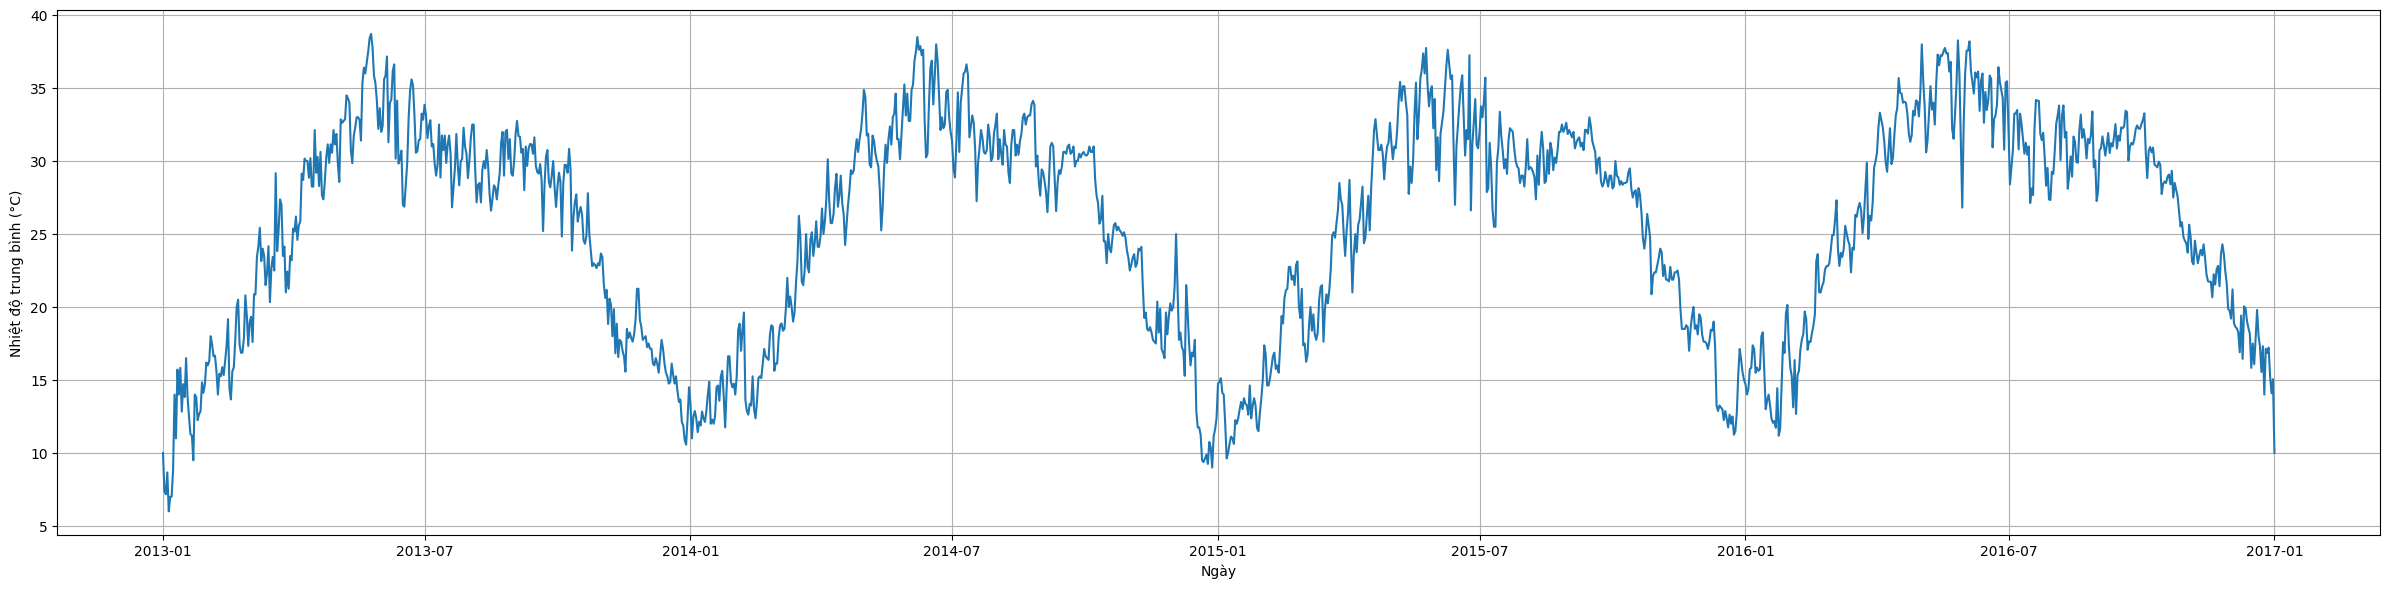
\includegraphics[width=0.90\textwidth]{images/TS_weather_meantemp.png}
        \caption{Nhiệt độ trung bình từng ngày}
        \label{fig:TS_weather_meantemp}
    \end{figure}
    \FloatBarrier

    Biểu đồ đường \ref{fig:TS_weather_meantemp} thể hiện sự thay đổi nhiệt độ trung bình (°C) theo thời gian. Từ biểu đồ, thời gian từ đầu năm 2013 đến cuối năm 2016, ta thấy mỗi năm đều có mô hình biến động tương tự, cho thấy tính chất thời vụ mạnh mẽ.

    \begin{figure}[htp]
        \centering
        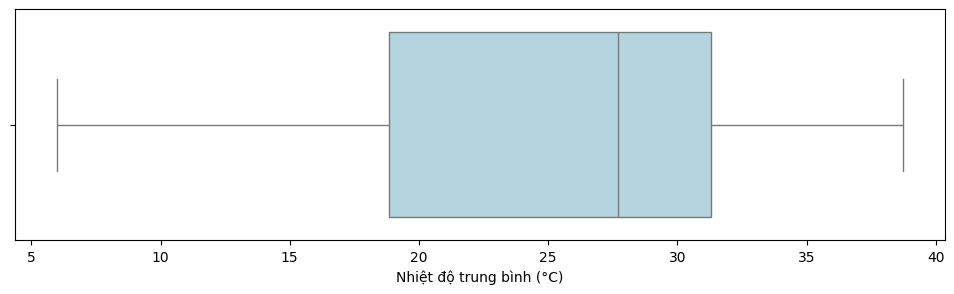
\includegraphics[width=0.90\textwidth]{images/TS_weather_boxplot_meantemp.png}
        \caption{Nhiệt độ trung bình}
        \label{fig:TS_weather_boxplot_meantemp}
    \end{figure}
    \FloatBarrier

    Biểu đồ \ref{fig:TS_weather_boxplot_meantemp} cho thấy phần lớn nhiệt độ nằm trong khoảng từ khoảng 19°C đến 32°C, với trung vị khoảng 28°C. Điều này cho thấy khí hậu nhìn chung khá ấm, với nhiệt độ trung bình thường nghiêng về mức cao. Không có điểm ngoại lệ rõ rệt, cho thấy nhiệt độ biến động trong phạm vi tương đối đều và ổn định

    \begin{figure}[htp]
        \centering
        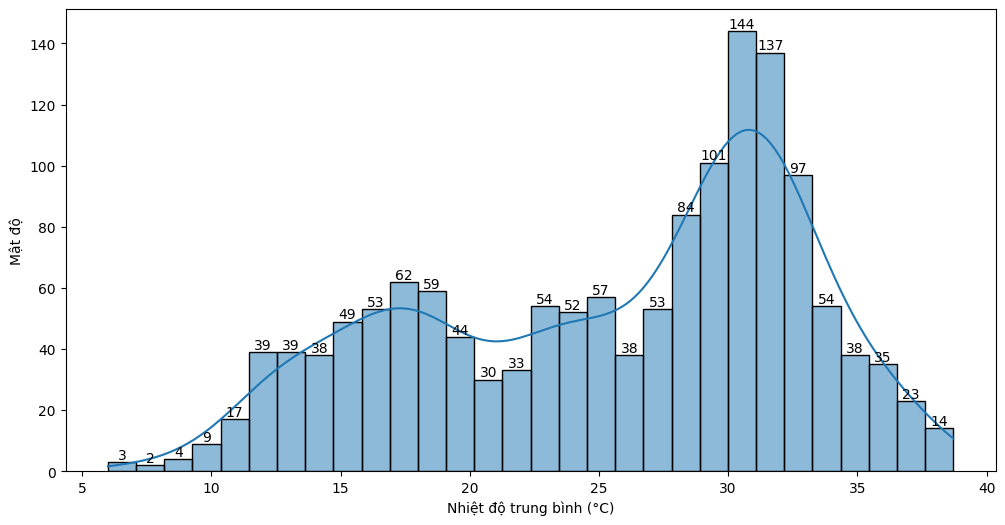
\includegraphics[width=0.90\textwidth]{images/TS_weather_hist_meantemp.png}
        \caption{Phân phối nhiệt độ trung bình}
        \label{fig:TS_weather_hist_meantemp}
    \end{figure}
    \FloatBarrier

     Biểu đồ \ref{fig:TS_weather_hist_meantemp} cho thấy phân phối nhiệt độ trung bình có dạng chuông, lệch trái, cho thấy khí hậu trong dữ liệu thiên về nhiệt độ nóng.

     \begin{figure}[htp]
        \centering
        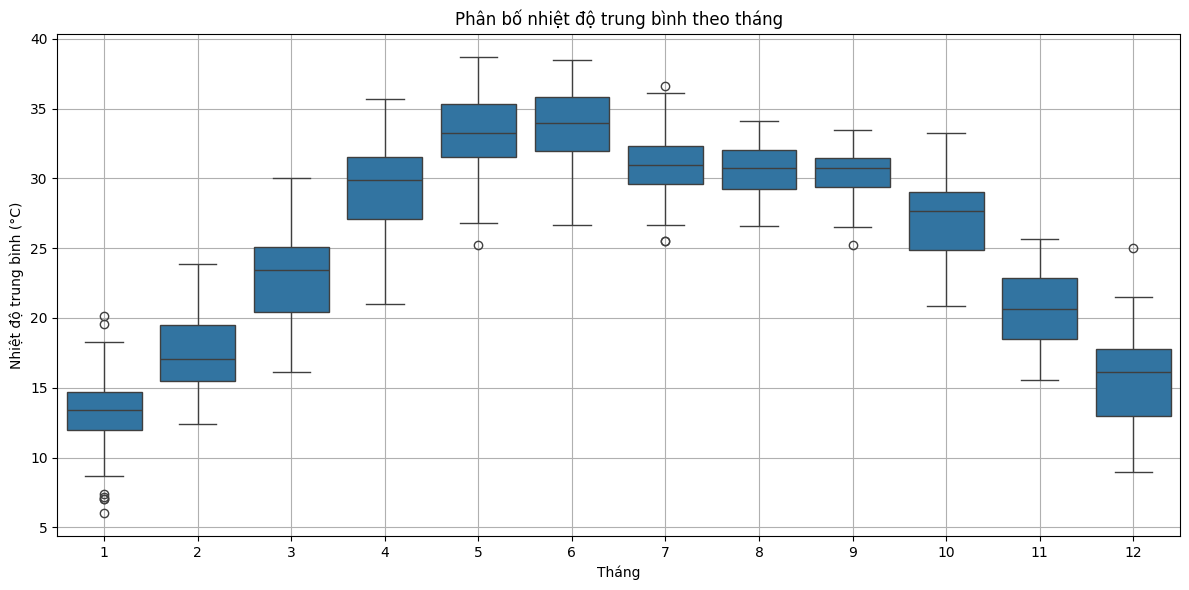
\includegraphics[width=0.90\textwidth]{images/TS_weather_boxplot_month_meantemp.png}
        \caption{Nhiệt độ trung bình các tháng}
        \label{fig:TS_weather_boxplot_month_meantemp}
    \end{figure}
    \FloatBarrier

    Biểu đồ \ref{fig:TS_weather_boxplot_month_meantemp} cho thấy sự phân bố nhiệt độ trung bình theo từng tháng trong năm, phản ánh rõ rệt tính chu kỳ của thời tiết. Từ tháng 1 đến tháng 6, nhiệt độ tăng dần, với đỉnh nằm ở tháng 5 và 6. Sau đó, từ tháng 7 trở đi, nhiệt độ bắt đầu giảm dần, đặc biệt rõ rệt từ tháng 10 đến tháng 12. Sự thay đổi này tạo nên dạng hình vòng cung điển hình cho chu kỳ mùa. Biên độ nhiệt trong các tháng mùa hè (tháng 4 đến 6) và mùa đông (tháng 1, 12) cũng lớn hơn, cho thấy thời tiết trong giai đoạn này biến động mạnh hơn. Ngược lại, các tháng giữa như tháng 8 và 9 ổn định hơn, với hộp hẹp và ít ngoại lệ.

    \begin{figure}[htp]
        \centering
        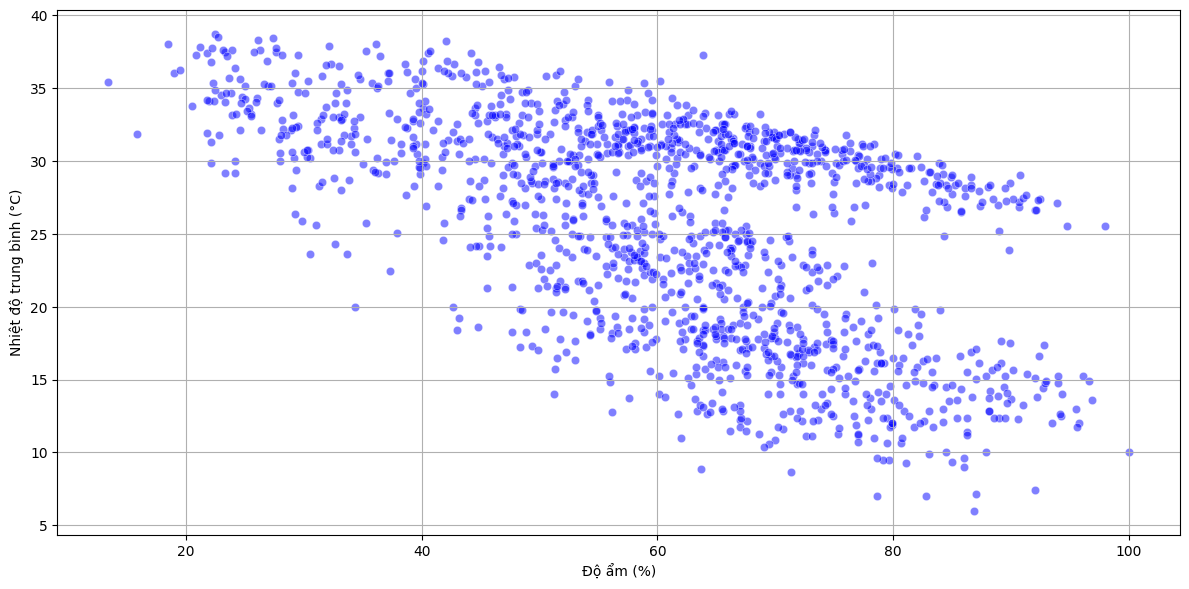
\includegraphics[width=0.90\textwidth]{images/TS_weather_meantemp_humid.png}
        \caption{Tương quan nhiệt độ - độ ẩm}
        \label{fig:TS_weather_meantemp_humid}
    \end{figure}
    \FloatBarrier

    Biểu đồ \ref{fig:TS_weather_meantemp_humid} thể hiện mối tương quan âm giữa hai biến. Mối quan hệ này phản ánh đặc điểm khí hậu phổ biến: khi trời nắng nóng khô thì độ ẩm thấp, còn những ngày mưa hoặc lạnh thường đi kèm độ ẩm cao

\subsubsection{Mô hình hóa dữ liệu}
    \paragraph{Cấu hình cài đặt} 
    \leavevmode

    Các mô hình sử dụng:

    \begin{itemize}
        \item \textbf{Linear Regression}: 

            \begin{lstlisting}[language=Python]
                LinearRegression()
            \end{lstlisting}

        \item \textbf{Random Forest Regressor}:

            \begin{lstlisting}[language=Python]
                RandomForestRegressor(
                    n_estimators=n_estimators, 
                    max_depth=max_depth, 
                    min_samples_leaf=min_samples_leaf
                )
            \end{lstlisting}

            khoảng hypertune tham số

            \begin{lstlisting}[language=Python]
                list_max_depth = [2, 3, 5, 10]
                list_n_estimators = [50, 100, 150, 200]
                list_min_samples_leaf = [1, 3, 5, 10]
            \end{lstlisting}.

        \item \textbf{XGBoost Classifier}:
            \begin{lstlisting}[language=Python]
                XGBRegressor(
                    n_estimators=n_estimators, 
                    max_depth=max_depth, 
                    reg_lambda=reg_lambda,
                    learning_rate=learning_rate,
                    reg_alpha=reg_alpha,
                )
            \end{lstlisting}

            khoảng hypertune tham số

            \begin{lstlisting}[language=Python]
                list_max_depth_xgb = [ 6, 7, 8]
                list_lambda = [0.5, 1, 2]
                list_learning_rate = [0.05, 0.1, 0.5]
                list_n_estimators_xgb  = [100, 150, 200]
                list_alpha = [0.5, 1]
            \end{lstlisting}.
        
    \end{itemize}

    Thuật toán data transform sử dụng: Standard Scaler.

    Chia tập dữ liệu huấn luyện: Train-Test: 80-20.

    \paragraph{Hồi quy nhiệt độ trung bình ngày 'meantemp'}
    \leavevmode

    Chuyển đặc trưng 'meantemp' về dạng sliding window để dự đoán hồi quy, thử nghiệm trên các khoảng: 3,7,14,30

    Kết quả:
    \begin{itemize}
        \item \textbf{Linear Regression}: 
        
            Mô hình tốt nhất:
            \begin{itemize}
                \item Khoảng sliding window: 14
            \end{itemize}

            \begin{table}[htbp]
            \centering
            \caption{Kết quả Linear Regression}
            \label{tab:weather-meantemp-lireg}
            \begin{tabular}{llrrr}
            \hline
             & Dataset & MAE & RMSE & MAPE \\
            \hline
            0 & Train & 1.206136 & 1.582341 & 5.355188 \\
            1 & Test & 1.225678 & 1.609280 & 4.539541 \\
            \hline
            \end{tabular}
            \end{table}
  
            
            \FloatBarrier

            \begin{figure}[htp]
                \centering
                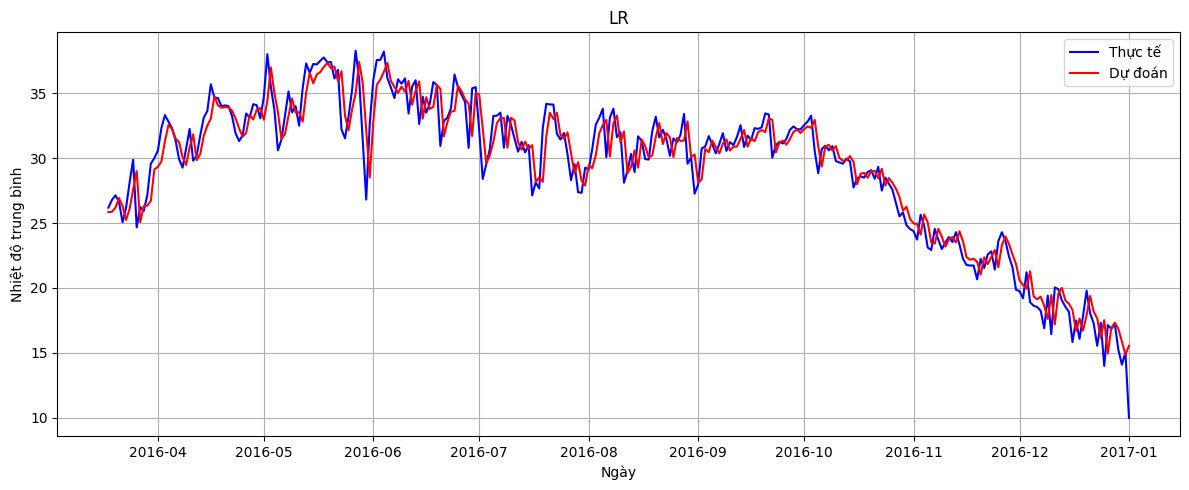
\includegraphics[width=0.90\textwidth]{images/TS_weather_pred_cmp_LR.png}
                \caption{Kết quả trên tập test Linear Regression}
                \label{fig:TS_weather_pred_cmp_LR}
            \end{figure}
        
            \FloatBarrier
            
        \item \textbf{Random Forest Regressor}:

            Mô hình tốt nhất:
            \begin{itemize}
                \item Khoảng sliding window: 14
                \item max\_depth: 10
                \item n\_estimators: 200
                \item min\_samples\_leaf: 5
            \end{itemize}

            \begin{table}[htbp]
                \centering
                \caption{Kết quả Random Forest Regressor}
                \label{tab:weather-meantemp-rf}
                \begin{tabular}{llrrr}
                \hline
                 & Dataset & MAE & RMSE & MAPE \\
                \hline
                0 & Train & 0.797399 & 1.072293 & 3.490075 \\
                1 & Test & 1.240903 & 1.602772 & 4.509175 \\
                \hline
                \end{tabular}
            \end{table}
            
            \FloatBarrier

            \begin{figure}[htp]
                \centering
                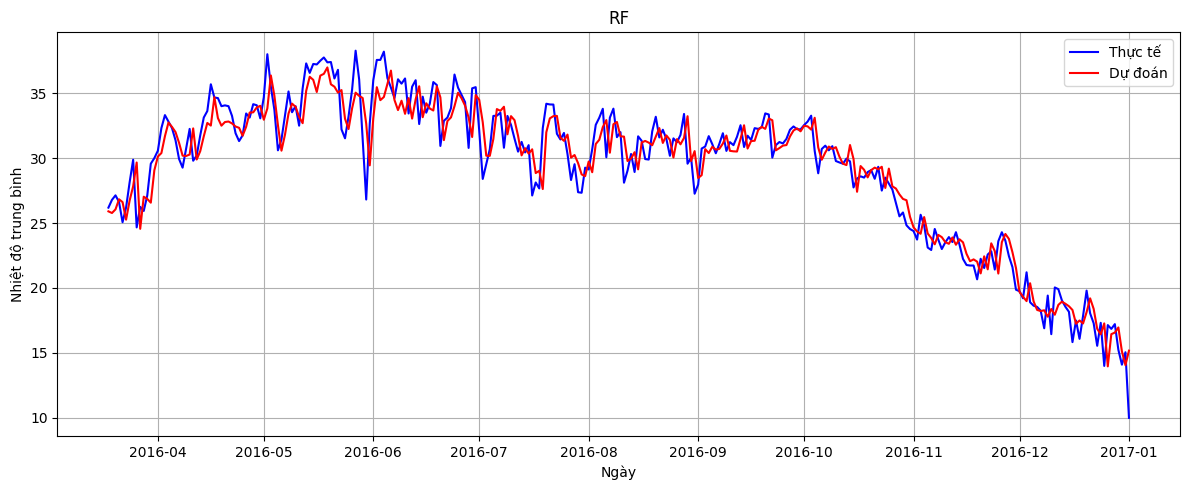
\includegraphics[width=0.90\textwidth]{images/TS_weather_pred_cmp_RF.png}
                \caption{Kết quả trên tập test RF Regressor}
                \label{fig:TS_weather_pred_cmp_RF}
            \end{figure}
            \FloatBarrier

        \item \textbf{XGBoost Regressor}:
        
            Mô hình tốt nhất:
            \begin{itemize}
                \item Khoảng sliding window: 7
                \item max\_depth: 6
                \item n\_estimators: 100
                \item reg\_lambda: 2
                \item reg\_alpha: 0.5
                \item learning\_rate: 0.05
            \end{itemize}

            \begin{table}[htbp]
                \centering
                \caption{Kết quả XGBoost Regressor}
                \label{tab:weather-meantemp-xgb}
                \begin{tabular}{llrrr}
                \hline
                 & Dataset & MAE & RMSE & MAPE \\
                \hline
                0 & Train & 0.851096 & 1.107114 & 3.817686 \\
                1 & Test & 1.301333 & 1.712462 & 4.686959 \\
                \hline
                \end{tabular}
            \end{table}

            \FloatBarrier

            \begin{figure}[htp]
                \centering
                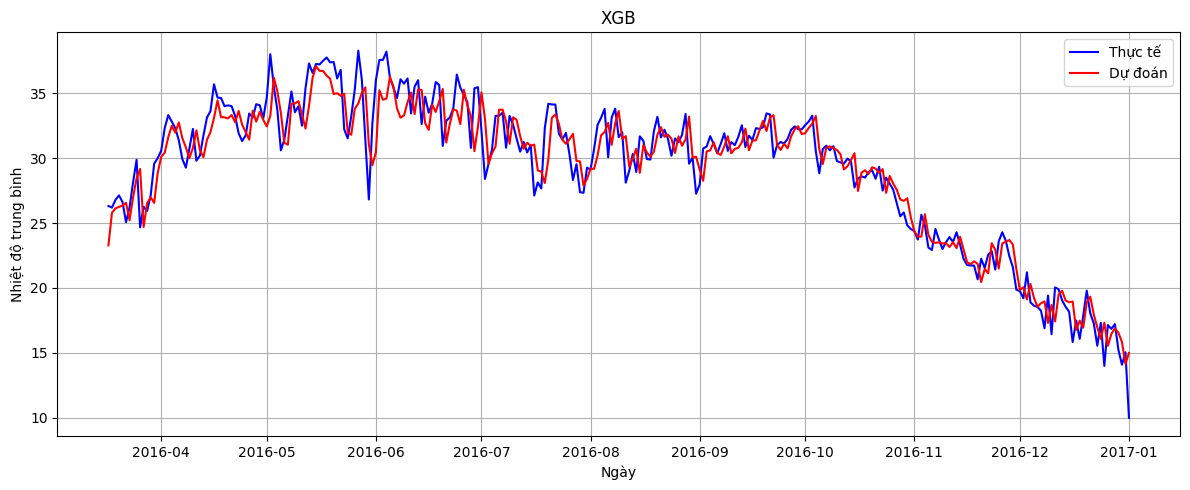
\includegraphics[width=0.90\textwidth]{images/TS_weather_pred_cmp_XGB.png}
                \caption{Kết quả trên tập test XGB Regressor}
                \label{fig:TS_weather_pred_cmp_XGB}
            \end{figure}
            \FloatBarrier
    \end{itemize}

    So sách các mô hình:

    \begin{table}[htbp]
        \centering
        \caption{So sánh kết quả các mô hình (và nghiên cứu liên quan)}
        \label{tab:weather-meantemp-compare}
        \begin{tabular}{|l|c|c|c|}
        \hline
        Model & MAE & RMSE & MAPE \\
        \hline
        Linear Regression & \textbf{1.225678} & 1.609280 & 4.539541 \\
        \hline
        Random Forest & 1.240903 & \textbf{1.602772} & \textbf{4.509175} \\
        \hline
        XGBoost & 1.301333 & 1.712462 & 4.686959 \\
        \hline
        CNN LSTM \cite{yunsuxiaozi} &   & 5.53722 &   \\
        \hline
        \end{tabular}
    \end{table}

    \FloatBarrier

    Random Forest đạt hiệu suất tổng thể tốt nhất với RMSE và MAPE thấp nhất, trong khi Linear Regression cho MAE thấp nhất. XGBoost xếp sau hai mô hình trên nhưng vẫn cho kết quả chấp nhận được. So với nghiên cứu trước sử dụng CNN LSTM \cite{yunsuxiaozi}, các mô hình hiện tại đều vượt trội rõ rệt về độ chính xác, đặc biệt là RMSE, cho thấy mô hình truyền thống có thể phù hợp hơn trong bài toán dự báo nhiệt độ trung bình với dữ liệu này. Mô hình đơn giản cho kết quả tốt hơn có thể do nhiệt độ trung bình các ngày đã đủ rõ ràng để các mô hình tuyến tính hoặc cây quyết định khai thác hiệu quả mà không cần kiến trúc học sâu. Tương tự đó cũng có thể lý do mô hình XGBoost phức tạp cho kết quả thấp hơn

\subsubsection{Kết luận}
    Trong phần này, nhóm đã tiến hành phân tích và xây dựng mô hình hồi quy trên dữ liệu thời tiết thành phố Delhi. Kết quả cho thấy các mô hình truyền thống như Linear Regression và Random Forest hoạt động hiệu quả hơn đáng kể so với mô hình học sâu CNN LSTM từ nghiên cứu trước. Random Forest là mô hình thể hiện tốt nhất tổng thể, đạt RMSE và MAPE thấp nhất trên tập kiểm tra, trong khi Linear Regression cho MAE thấp nhất.